%% Template for ENG 401 reports
%% by Robin Turner
%% Adapted from the IEEE peer review template

%
% note that the "draftcls" or "draftclsnofoot", not "draft", option
% should be used if it is desired that the figures are to be displayed in
% draft mode.

\documentclass[peerreview]{IEEEtran}
\usepackage{cite} % Tidies up citation numbers.
\usepackage{url} % Provides better formatting of URLs.
\usepackage[utf8]{inputenc} % Allows Turkish characters.
\usepackage{booktabs} % Allows the use of \toprule, \midrule and \bottomrule in tables for horizontal lines
\usepackage{graphicx}
\usepackage{amsmath}
\usepackage[super]{nth}


\hyphenation{} % Corrects some bad hyphenation 



\begin{document}
%\begin{titlepage}
% paper title
% can use linebreaks \\ within to get better formatting as desired
\title{Exploring Transformers Outside of NLP}


% author names and affiliations

\author{Arsyi Syarief Aziz \\
Computer Science Study Program\\
Department of Mathematics\\
Universitas Hasanuddin\\
}
\date{25/4/15}

% make the title area
\maketitle
\tableofcontents
\listoffigures
\listoftables
%\end{titlepage}

\IEEEpeerreviewmaketitle
\begin{abstract}
The transformer is a robust neural network architecture that has surpassed the performance of RNNs, CNNs, and even ensemble models in machine translation. In addition to being performant in NLP, previous research has shown that transformers can also work in other domains. To further explore this capability, the transformer was tested in its ability to complete two tasks: to reverse a sequence and to identify the anomaly image in an image set. The architecture's performance on these tasks was assessed based on its accuracy in producing the expected output. The results of the experiments showed that transformers were capable of completing both tasks accurately. In the first task, the transformer produced an accuracy of 100\% in both its training set and test set, and in the second task, the transformer produced an accuracy of 96.35\% and 94.41\% in its training set and test set, respectively.

\end{abstract}

\section{Introduction}

This report discusses about the capability of transformers outside of the natural language processing (NLP) domain.

The transformer in this report is defined as a robust neural network architecture that has been proven perform well in the domain of natural language processing. It has surpassed the performance of RNNs, CNNs, and even ensemble models in machine translation 
\cite{vaswani_2017}. The high performance can be attributed to its use of attention mechanisms, which allows the model to be parallelized and learn long-term dependencies \cite{vaswani_2017}.

Not only are transformer performant in NLP, but they have also been shown to work in other domains, such as computer vision \cite{dosovitskiy_2021}. In order to explore the capability of this architecture, I have conducted experiments using transformers to complete tasks based on two different types of data, which include sequenced data and set data. These data types were specifically chosen because they can be expressed as a sequence; allowing the attention mechanism in transformers to be utilized.

More details about the experiments are elaborated in the following sections.


\section{Problem Definition}
The experiments conducted for this report include two problems, one to test the performance of the transformer in processing sequenced data and another to test its performance on set data.

In the first problem, the transformer was given a random sequence of numbers of length $N$. The task of the transformer was to reverse the sequence of data, such that a sequence that might originally be 123456789 is transformed into the expected output of 987654321.

For the second problem, a set of $N$ images was sampled from the CIFAR100 dataset. In each set of images, there were $N-1$ images of the same category and $1$ image that is of a different category, which is called an anomaly. Based on the set of data mentioned previously, the task of the transformer was to correctly identify the anomaly image among the other $N-1$ images.

\begin{figure}[!h]
\centering

\includegraphics[width=0.8\columnwidth]{imageset} 
\caption{A set of 10 images from the CIFAR100 dataset. Pictures one to nine (from the left) are images of trees. Picture ten is an image of a volcano (the anomaly).}
\label{fig_image_set}
\end{figure}

% Note that IEEE typically puts floats only at the top, even when this
% results in a large percentage of a column being occupied by floats.

\section{Proposed Solution}
As mentioned in a previous section, the problems were solved using transformers. 

A transformer itself is a neural network architecture that utilizes attention to understand the correlations in a sequence. The attention mechanism usually consists of four components. First is the query, which is a feature vector that describes what a model is looking for in a sequence. Second are the keys, which are feature vectors that roughly describe what an element is offering. Third are the values, which are feature vectors indicating the value of an element. Last is the score function, $f_{attn}$, which is a function that takes a query and key as input, and outputs a score. These four components are used to calculate a weighted average defined in the mathematical notation below.

$$
\alpha_i = \frac{\exp(f_{attn}(key_i, query))}{\sum_j{\exp(f_{attn}(key_i, query)})}, 
$$

$$
out=\sum_i{\alpha_i \cdot \text{value}_i}.
$$

The attention mechanism applied to transformers is called self-attention, or more specifically, scaled dot product attention. This mechanism utilizes the dot product as the score function and a scaling factor, $d_k$, to scale the score value. From this description, we can more specifically define the mathematical formula for attention in transformers to the following equation.
$$
\textrm{Attention}(Q, K, V) = \textrm{Softmax}(\frac{QK^T}{\sqrt{d_k}})V.
$$

To further extend the attention mechanism, transformers allow multiple attentions to be used. This feature is called multi-head attention and it allows a model to attend to multiple aspects of a sequence. It works by transforming a query, key and value into $h$ sub-queries, sub-keys, and sub-values, which are then passed through $h$ scaled dot product attentions, called heads. These heads are concatenated before being multiplied by a weight matrix to form multi-head attention. 

$$
Multihead(Q, K, V) = Concat(head_1, \dots, head_h)W^O.
$$

Based on the defined attention mechanism above, transformers are built upon an encoder-decoder structure. The encoder part consists of $N$ identical blocks arranged in a sequence, called encoder blocks. These encoder blocks are built upon a single multi-head attention block, followed by a single feed-forward network block. The output of each of these blocks are added with their respective inputs through a residual connection and are normalized. For the decoder part, the structure is similar to the encoder, but it has an additional masked multi-head attention block that processes the output of an encoder. This additional block functions to prevent positions in the input sequence from attending to subsequent positions \cite{vaswani_2017}. Fig. \ref{fig_transformer} best describes the architecture.
\begin{figure}[!h]
\centering
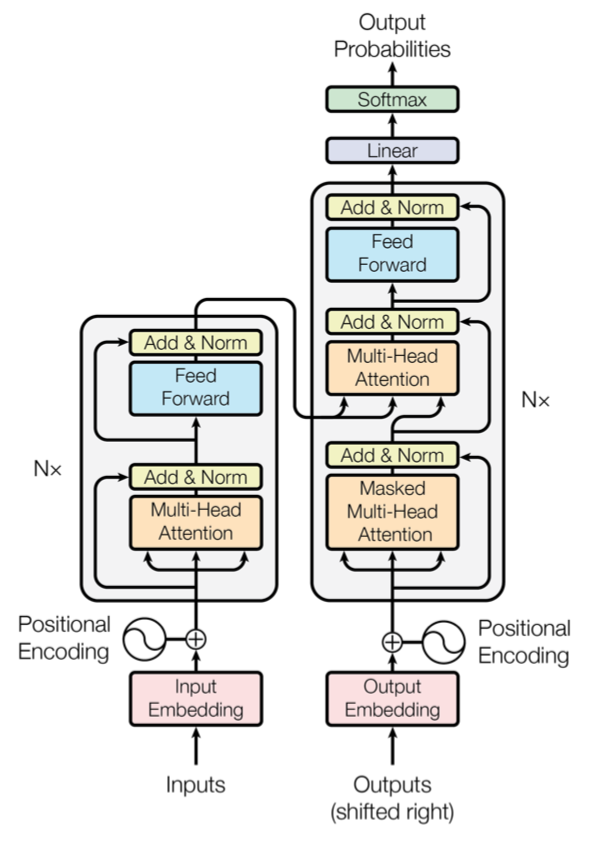
\includegraphics[width=0.8\columnwidth]{transformer} 
\caption{The transformer architecture.}
\label{fig_transformer}
\end{figure}

\section{Criteria for Assessing Solutions} \label{sec:criteria}
The criteria used to assess the transformer's solution to a given problem is its accuracy in predicting the expected output. This accuracy metric is calculated slightly differently in the two experiments. In the sequence reversal experiment, accuracy is calculated as the percentage of predicted elements in the correct position. Meanwhile, in the set anomaly experiment, accuracy is calculated as the percentage of correctly identified anomalies. 

\section{Research Methodology}
The experiments in this report were conducted using encoder-based transformer models, which are models that contain an encoder, but do not contain a decoder. This was chosen to simplify the implementation of the architecture, and has been proven by research \cite{dosovitskiy_2021}\cite{devlin_2018} to work in some tasks. 

During training, the models used learning rate warm-up scheduling, which helps to improve their performance \cite{liu_2020}. This scheduling method works by gradually increasing the learning rate of a model from 0 to a specified learning rate after a few iterations. The specific learning rate warm-up method utilized in the models is called the cosine warm-up scheduler \cite{vaswani_2017}.

Because both experiments were conducted on two different data types with different properties, two different methods had to be used. To explain these methods, I will first explain about the sequence reversal experiment and then explain about the anomaly detection experiment.

In the sequence reversal experiment, the task of the model was to reverse an input sequence. To complete this task, the model needs to understand the positions of the elements in a sequence. However, due to transformers being permutation-invariant \cite{naseer_2021}, it cannot immediately differentiate positions in a sequence without positional information. For this reason, positional encoding was embedded into an input sequence before passing it to the transformer. The positional encoding used in the model consists of a sine and cosine function, defined in \cite{vaswani_2017}. After positional encoding was embedded, the encoded sequence was passed through a transformer model to reverse it. This model consisted of 32 hidden layers, 1 head, and 1 encoder block. Additionally, the model was trained with a learning rate of 0.0005, and a warm-up period of 50 epochs.

In the set anomaly task, the goal was to identify the anomaly image in an image set. In order to do this, a CNN was first used to extract high-level features of each image in the image set. After extracting these features, the features were then passed into the transformer model without positional encoding to identify the anomaly. Unlike the first experiment, positional encoding was not needed in this experiment because the position of an anomaly in an image set is not important. In terms of the hyper-parameters of the model, it included 256 hidden layers, 4 heads, and 4 encoder blocks. On top of this, the model was trained with a learning rate of 0.0005, and a warm-up period of 100 epochs.

\section{Analysis and Interpretation}
% Example of a table from http://www.latextemplates.com/template/professional-table
After conducting the experiments, I gathered the following results. 


\begin{table}[h] 
\centering 
\begin{tabular}{l c c}
\toprule 
& \multicolumn{2}{c}{Accuracy} \\ 
\cmidrule(l){2-3} 
Experiment & Train & Test\\ 
\midrule
Sequence Reversal & 100\% & 100\%\\
Anomaly Detection & 96.35\% & 94.41\%\\ 
\bottomrule
\end{tabular}
\smallskip 
\caption{Experiment results} 
\label{tab:experiment results}
\end{table}

Based on Table \ref{tab:experiment results}, it appears that the transformer model was able to complete the two tasks with great accuracy. Specifically speaking, in the first task, the model correctly reversed 100\% of the input sequences in both the train and test set. Meanwhile, for the anomaly detection task, the model was able to correctly identify 96.35\% of the anomalies in the training set and  94.41\% of the anomalies in the test set.

To understand how the model was able to achieve such high accuracy, I will show the attention maps of the model in both tasks.

First is the attention map for the sequence reversal task. In Appendix. \ref{App:reversal_attention_map}, we can see that the model determines the elements of the output sequence by attending to the element in the opposite index. For example, we can see that the element in index 0 attends to the element in index 15, the element in index 1 attends to an element in index 14, the element in index 2 attends to an element in index 13, and so on. This is similar to how we humans would usually approach this problem.

Next is the anomaly detection task. Fig. \ref{anomaly_correct} shows an image set where the anomaly was identified correctly as the \nth{10} image, and Appendix. \ref{App:anomaly_attention_map_correct} shows its attention map. In the attention map, we can see that the multi-head attention layer focuses on the \nth{10} image in heads 1, 2, 3, and 4 of layer 2 and head 1 of layer 3. Meanwhile, in layer 4, all of the heads completely ignore the \nth{10} image. This indicates that image 10 is the anomaly. In another example, Fig. \ref{anomaly_correct} shows an image set where the model incorrectly identifies the \nth{8} image as the anomaly, and Appendix. \ref{App:anomaly_attention_map_incorrect} shows its attention map. From the attention map, we can see that the model's attention is pretty spread out, thus it hard to interpret. However, if we view the probabilities of each image, as seen in Table \ref{tab:probabilities}, we can see that the model focuses on images 6, 8, and 10 (image 10 being the anomaly). Despite focusing on the correct image, the model mistakenly predicts image 8 as the anomaly, as indicated by its high probability. This error could be attributed to image 8 being the only image with a building in the background.

\begin{table}[h] 
\centering 
\begin{tabular}{l l}
\toprule 
 & Probabilities\\ 
\midrule
Image 1 & 0.07\% \\ 
Image 2 & 00.11\% \\ 
Image 3 & 0.07\% \\
Image 4 & 0.11\% \\
Image 5 & 0.17\% \\
Image 6 & 23.27\% \\ 
Image 7 & 0.16\% \\
Image 8 & 48.91\% \\
Image 9 & 0.10 \% \\ 
Image 10 & 27.04\%\\
\bottomrule
\end{tabular}
\smallskip 
\caption{Probabilities in the anomaly detection task (incorrect identification example)} 
\label{tab:probabilities} 
\end{table}


\begin{figure}[!h]
\centering
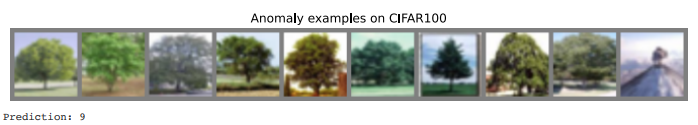
\includegraphics[width=1\columnwidth]{anomaly_correct} 
\caption{An image set of which the anomaly was correctly identified.}
\label{anomaly_correct}
\end{figure}

\begin{figure}[!h]
\centering
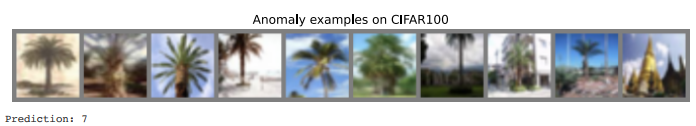
\includegraphics[width=1\columnwidth]{anomaly_incorrect} 
\caption{An image set of which the anomaly was incorrectly identified.}
\label{anomaly_incorrect}
\end{figure}


\section{Conclusions and Recommendations}
Based on the findings, it can be concluded that transformers perform well in both the sequence reversal task and anomaly detection task. This is further proof that transformers are capable of completing tasks outside of the NLP. Not only that, the findings have also shown that attention is capable of finding hidden correlations in data. By extending the attention mechanism to several heads, a transformer model is able to attend to several elements in a sequence, thus helping the model to better understand the hidden correlations.

Following this conclusion, I highly recommend using transformers in tasks related to sequence reversal and anomaly detection as they have demonstrated a high level of accuracy in the experiments.

\newpage
\appendices
\section{An example attention map in the sequence reversal task} \label{App:reversal_attention_map}
\begin{figure}[!h]
\centering
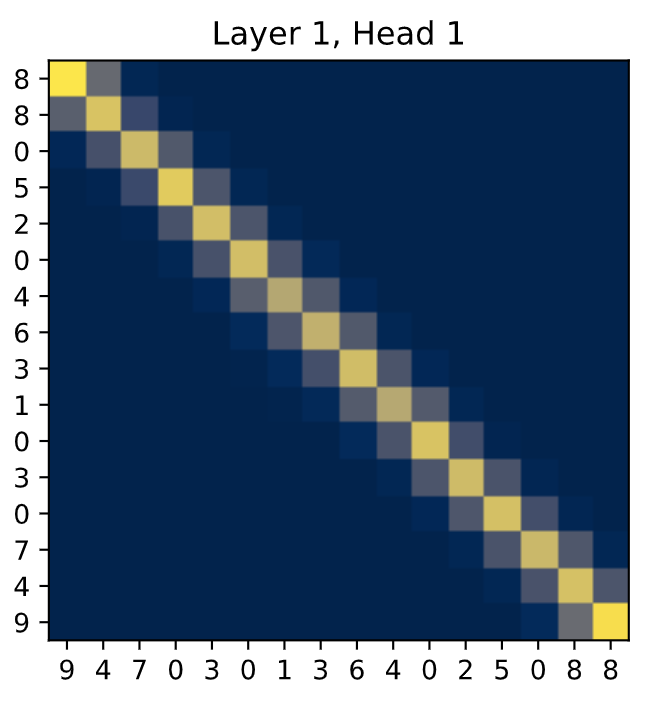
\includegraphics[width=0.8\columnwidth]{reversal_attention_map} 
\end{figure}
\section{An example attention map in the anomaly detection task (correct identification)} \label{App:anomaly_attention_map_correct}
\begin{figure}[!h]
\centering
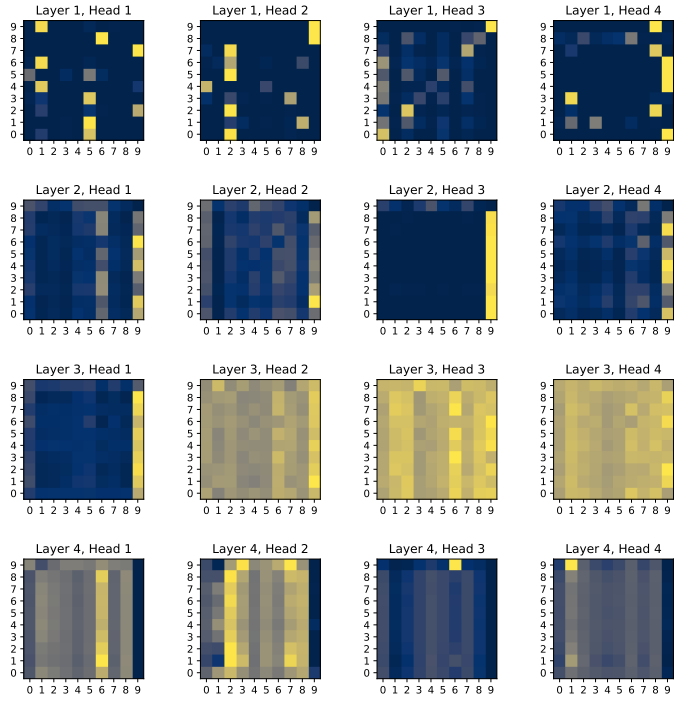
\includegraphics[width=1\columnwidth]{anomaly_attention_map_correct.png} 
\end{figure}
\newpage
\section{An example attention map in the anomaly detection task (incorrect identification)} \label{App:anomaly_attention_map_incorrect}
\begin{figure}[!h]
\centering
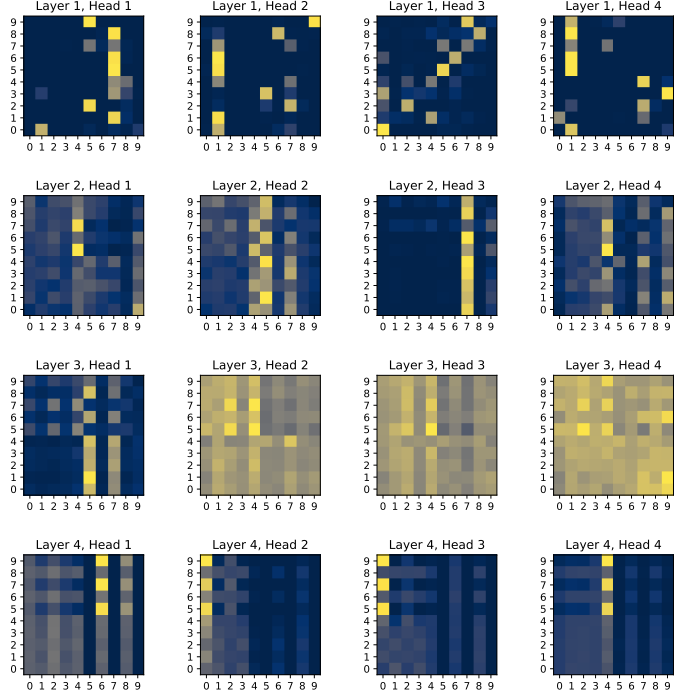
\includegraphics[width=1\columnwidth]{anomaly_attention_map_incorrect.png} 
\label{anomaly_attention_map_incorrect}
\end{figure}

\begin{thebibliography}{1}

\bibitem{vaswani_2017}
A. ~Vaswani, N. ~Shazeer, N. ~Parmar, J. ~Uszkoreit, L. ~Jones, A. N. ~Gomez, Ł. ~Kaiser, and I ~Polosukhin, "Attention is all you need", in Advances in Neural Information Processing Systems. 2017.

\bibitem{dosovitskiy_2021}
A. Dosovitskiy, L. Beyer, A. Kolesnikov, D. Weissenborn, X. Zhai, T. Unterthiner, M. Dehghani, M. Minderer, G. Heigold, S. Gelly, J. Uszkoreit, and N. Houlsby, "An image is worth 16x16 words: Transformers for image recognition at scale", in the International Conference on Learning. 2021.

\bibitem{devlin_2018}
J. Devlin, M. Chang, K. Lee, and K. Toutanova, "BERT: Pre-training of Deep Bidirectional Transformers for Language Understanding", arXiv preprint arXiv:1810.04805. 2018. 

\bibitem{liu_2020}
L. Liu, H. Jiang, P. He, W. Chen, X. Liu, J. Gao, and J. Han, "On the Variance of the Adaptive Learning
Rate and Beyond", in the International Conference on Learning. 2020. 

\bibitem{naseer_2021}
M. Naseer, K. Ranasinghe, S. Khan,
M. Hayat, F. S. Khan, and M. Yang, "Intriguing Properties of Vision Transformers", in Neural Information Processing Systems. 2021.
\end{thebibliography}



\end{document}


